\cleardoublepage


\chapter{Natural Language Processing}


Natural language processing (NLP) is a subfield of linguistics, computer science, information engineering and artificial intelligence, which is devoted to the engineering of computational models and processes to give the ability of human language understanding to computers. \cite{Khurana2018}  \par

Human language is extremely complex and rarely precise, to understand it is to understand not only the words, but the concepts and how they are linked together in order to create meaning. This makes NLP one of the most difficult tasks in computer science. \par

NLP consists in two major components, Natural Language Understanding (NLU) and Natural Language Generation (NLG).  \par

\begin{figure}[htb]
    \centering
    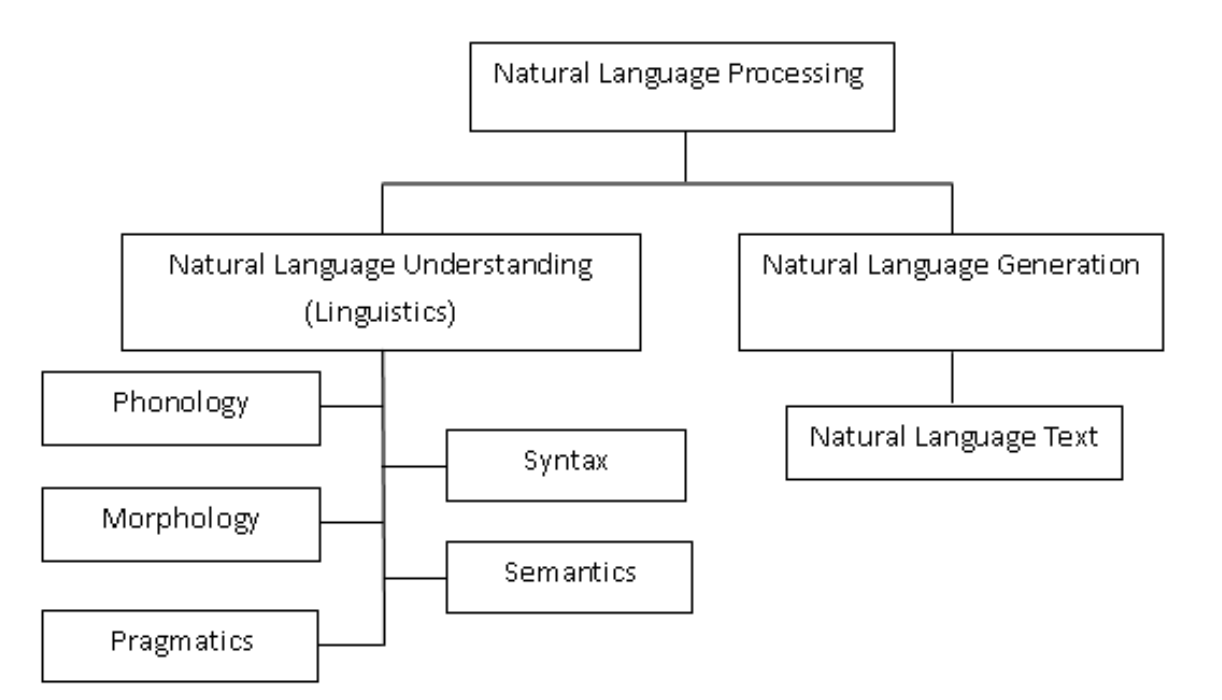
\includegraphics[scale = 0.25]{Sections/3StateOfTheArt/3_images/NLP_diagram.png}
    \caption{Classification of NLP. \cite{Khurana2018}}   
\end{figure}



Work in NLP can be divided in two broad sub-areas: core areas and applications area. The core areas address fundamental problems such as segmentation of meaningful components of words, syntactic processing, semantic processing and morphological processing \cite{Otter2018}. Currently, some applications for NLP are Machine Translation, Email Spam detection, Information Extraction, Personal Assistants (i.e Siri, Google Assistant), Chat bots, etc.  \par 

To perform translation, text summarization, image captioning, or any other linguistic task, there must be some understanding of the underlying language. This understanding can be broken down into at least 4 main areas : language modeling, morphology, parsing, semantics. \par 

Language modeling is the determination of the meaning of words and which words follow which. \par

Morphology is the study of how words themselves are formed, by considering the root of the word, it's suffixes and prefixes, gender, plurality, etc.

Parsing considers which words modify others. \par

Semantics is the study of the meaning of words by taking into account the meaning of individual words  and how they relate and modify others. \cite{Otter2018} \par 



\section{Numerical Representation of Text}


\par Machine learning algorithms and most of all deep learning architectures are incapable of processing strings and text, this is because they require numbers as an input. \cite{Vidhya2017} A human can easily tell that the word "dog" and the word "cat" are identical, since they both represent an animal, however a computer would answer that they are completely different things since all the letters in those words are different. 

    \subsection{Word Embeddings}

    \par The dominant approach to solve this problem is the usage of word embeddings, which is a type of word representation that allows words with similar meaning to have a similar representation by mapping a set of words, or phrases in a vocabulary, to vectors of numerical values. 

    \par  Word embedding methods learn a real-valued vector representation for a predefined fixed size vocabulary from a corpus  of text. \cite{Brownlee2017}  
   
    \par A vector representation of a word may be a one-hot encoded vector where 1 stands for the position where the word exists and 0 everywhere else. 
    
    \par As an example the sentence   ”Word Embeddings are Word converted into numbers” can be convert to a dictionary in this form : [‘Word’,’Embeddings’,’are’,’Converted’,’into’,’numbers’]. The vector representation of the word“numbers” in this format according to the above dictionary is [0,0,0,0,0,1] and of the word "converted" is [0,0,0,1,0,0]. This is considered to be the most simple method to represent words in vector forms. \cite{Vidhya2017}
    \par An image showcasing this example is shown below.
    
    
    \begin{figure}[htb]
        \centering
        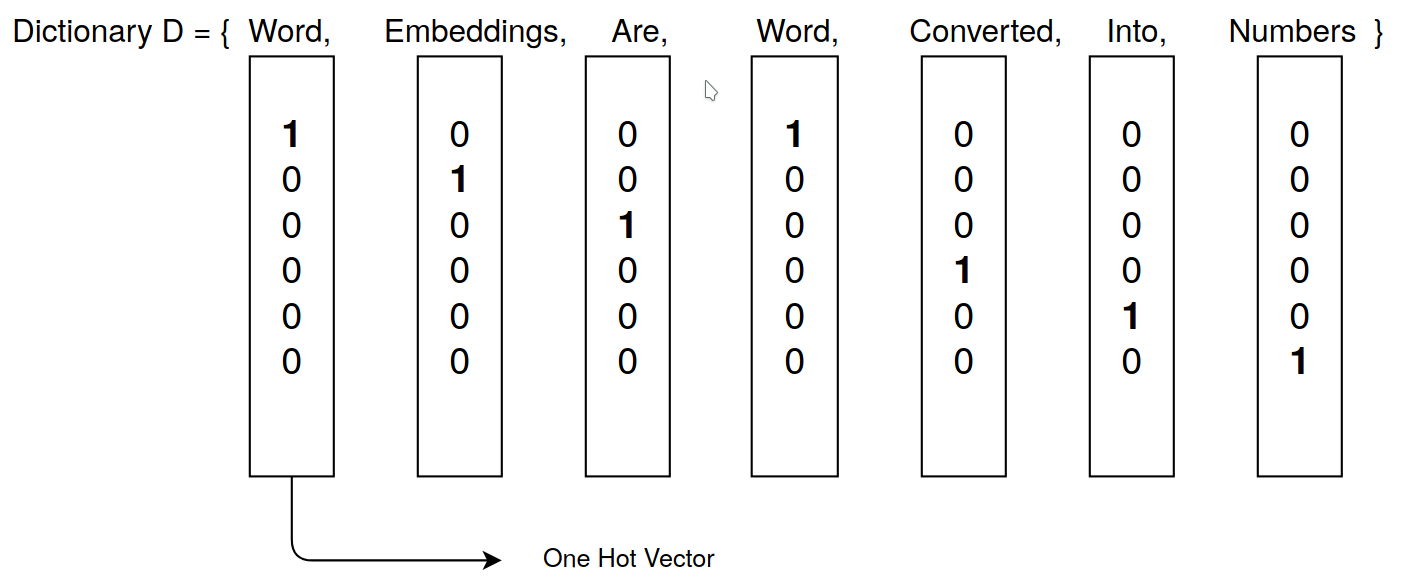
\includegraphics[scale = 0.25]{Sections/3StateOfTheArt/3_images/one_hot_encoding.png}
        \caption{Example of text representation by one-hot vector.}   
    \end{figure}
    
    
    

 

    \newpage

    \subsection{Static Word Embedding Models}
    \label{sec:static}
    \par This section introduces some common static word embedding models to learn word embeddings from text.


    \par Static word embedding have the fundamental problem which is they generate the same embedding, in different contexts, for the same word, failing to capture the polysemy of the word. This is due to the fact that each word has a single vector, regardless of context. \cite{Mikolov2013}  
   

    \par As an example, having these two phrases:

    \begin{itemize}
        \item "The Apple Company is the one who produces iPhones."
        \item "This apple is delicious."
    \end{itemize}

    \par In this case, the word "Apple" has two different meanings, being one a company and the other a fruit, however for static word embedding models the word representation for "Apple" would be the same, since they fail to capture the meaning of the word. \cite{Batista2018}

   
        \subsubsection{Word2Vec}

        \par Developed by Tomas Mikolov, et al. at Google in 2013, Word2Vec is a two-layer neural network that processes text by "vectorizing" words with the purpose of grouping vectors of similar words together in vectorspace. The way Word2Vec detects those similarities is by creating vectors that are distributed numerical representations of word features, without human intervention.


        \par In a regular one-hot encoded vector, all words have the same distance between each other, even though their meanings are completely different.

        \begin{figure}[htb]
            \centering
            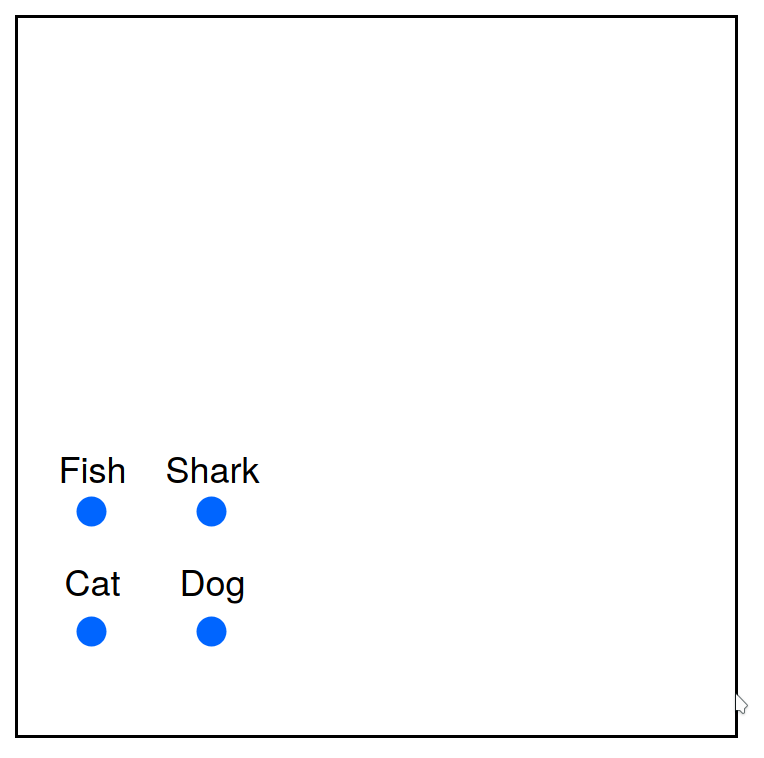
\includegraphics[scale = 0.1]{Sections/3StateOfTheArt/3_images/one_hot_ex.png}
            \caption{One-hot encoding resulting vector. \cite{word2vec_explained}} 
        \end{figure}


        \par Using Word2Vec, the resulting vector is able to  maintain context.


        \begin{figure}[htb]
            \centering
            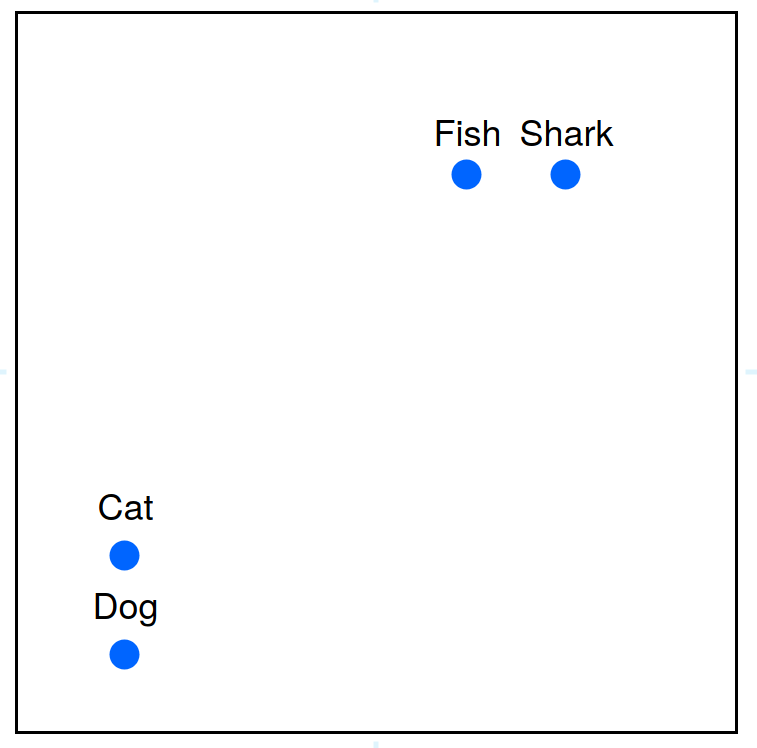
\includegraphics[scale = 0.1]{Sections/3StateOfTheArt/3_images/word2vec_encode.png}
            \caption{Word2Vec encoding resulting vector. \cite{word2vec_explained}}
        \end{figure}

        
        \par Word2Vec is capable of making accurate guesses, based on past appearances, of a word's meaning. 

        \par The output of Word2Vec is a vocabulary in which each item has a vector attached to it, which can be fed into a deep-learning net or simply queried to detect relationships between words.

        \par Word2Vec is composed of two different models, CBOW (Continuous Bag of words) which predicts a word given its context and Skip-Gram which predicts context given a word. \cite{Mikolov2013} \cite{Wiki}

        

        \begin{figure}[htb]
            \centering
            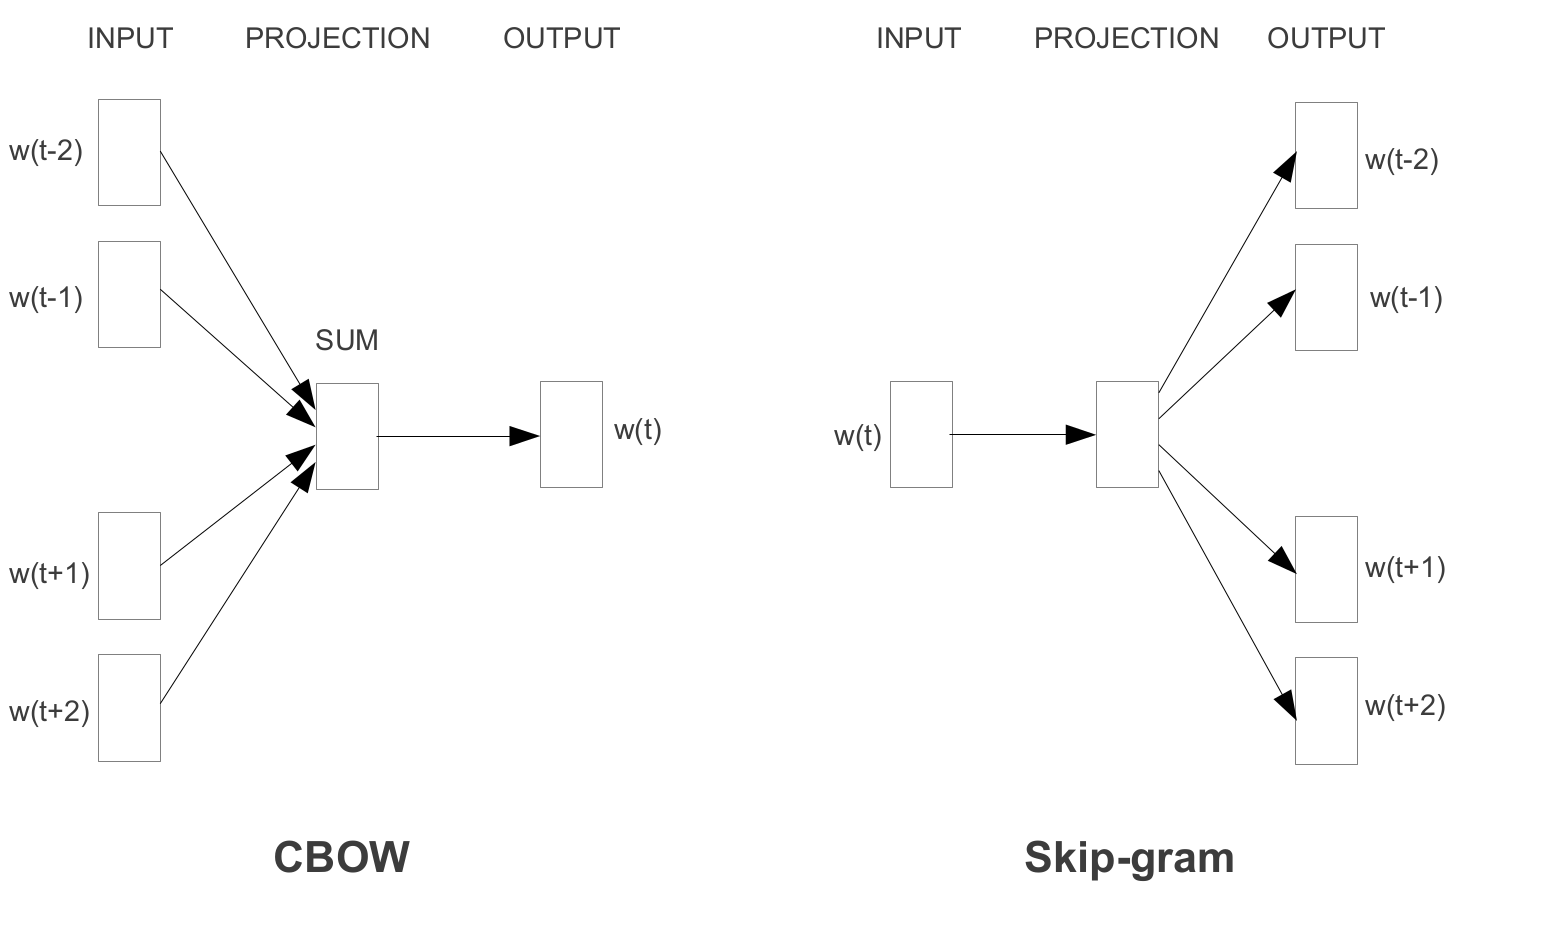
\includegraphics[scale = 0.15]{Sections/3StateOfTheArt/3_images/Cbow_Skip.png}
            \caption{CBOW model and Skip-Gram model. \cite{Mikolov2013}} 
        \end{figure}

        
        \subsubsection{GloVe}

        \subsubsection{fastText}
    
    \subsection{Contextualized Word Embedding Models}

        \par This section introduces some common contextualized word embedding models to learn word embeddings from text.
        
        \par Contextualized words embeddings aim at capturing word semantics in different contexts to address the issue of polysemous and the context-dependent nature of words \cite{Batista2018}. So, in theory, for the example given in  \ref{sec:static}, these models would be able to distinguish the different usage of the word Apple to represent the fruit or the company.



        \subsubsection{COVE}
        \subsubsection{ELMO}
        \subsubsection{BERT}
        \subsubsection{XLNet}
        

       
\section{Available NLP libraries}


        \subsection{SpaCy}
        
        \par SpaCy is a free, open-source library for advanced natural language processing written in Python and Cython published by Explosion AI. It was designed specifically for production use and to help in the building of applications that process and "understand" text data. Some use cases for this specific library are to build information extraction or natural language understanding systems, or to pre-process text for deep learning. \cite{Spacy2017}


        \subsection{Gensim}

        \par Gensim is a Natural Language Processing open-source library for unsupervised topic modeling (a technique to extract the underlying topics from large volumes of text)  and for natural language processing


        \subsection{Natural Language ToolKit}

        \subsection{Stanford Core NLP}

        \subsection{Flair}

        \subsection{Pattern}